\section*{Composition and Face Detection}

We analyze film composition at two levels of abstraction: the \emph{frame} and the \emph{sequence}.  A frame is a single image produced by a camera in the film.  A sequence is a series of camera shots, where each shot is an unbroken series of frames produced by a single camera.  Frame composition and sequence structure provide a sufficient basis upon which to begin analysis, are explicitly defined, and are directly related to the work of the cinematographer.

To analyze frame composition and sequence structure we first classify each frame and then use patterns in the sequence of frame classes to determine sequential structure.  We restrict our classification of frame composition in this work to frame orientations which  

\subsection{Frame Composition}

We restrict our description of the frame composition to population, zoom
and position of actors in the frame. Other visual elemements, such as
non-human points of interest (e.g. a car in the midst of
a chase sequence) can be as or more important than actors in a given frame;
 however, actors are at the core of most motion-pictures, and are therefore a good point of
 entry for better automatic understanding frame composition.

To detect the population, zoom and position of actors in each frame we 
use a state-of-the-art face detector~\cite{mathias_face_2014}.  

\subsubsection{Population}
The population of a frame is defined as the number of faces visible. We consider a face to be valid whether it is an actor, a photograph, a movie-within-a-movie or some other indirect face. A face is also valid regardless of minor occlusions (e.g. hair or partial masks) and orientation (e.g. face is oriented away from the camera). A face is invalid if it is non-human (e.g. animals, monsters, drawings, or CGI renderings). 

%--------------------------------------------------------------------------------

\subsubsection{Zoom}
Zoom is the perceived distance between camera and actor. This is typically classified by how much of the actor is visible within the shot. Figure \ref{fig:zoomClass} shows the seven commonly used zoom classifications. We stick to the traditional nomenclature of 'shot', though we are classifying frames. The classifications  are, in descending order of 'closeness':


%%%%%%%%%%%%%%%%%%%%%%%%%%%%%%
\textbf{Extreme Close-Up - ECU} In these frames, the camera is so close to the actor that the audience cannot see the actor's entire face. This creates a frame in which the actor's face exceeds the size of the frame.

\textbf{Close-Up - CU} In a Close-Up, the viewer can see the actors entire face, and perhaps their neck and trapezius, however the shoulders are typically not in the frame. 

\textbf{Medium Close-Up - MCU} Between a medium shot and a close-up, these frames contain the actor's entire face as well as their neck, shoulders, and clavicular region. 

\textbf{Medium Shot - MS} A Medium Shot shows the actor from the abdomen and above. 

\textbf{Medium Long Shot - MLS} These frames contain most, but not all of an actor's body. The shots typically contain some or all of the leg, but will not show the feet. A common location to cut-off the actor in these shots is at the knees. Cutting at mid-thigh, the knees, or mid-shin is considered more visually appealing than cutting at the ankles \cite{arijon_grammar_1991}.

\textbf{Long Shot - LS}In a Long Shot, the actor's entire body, from head to toe, is visible. In these frames, the actor is generally still in the forefront of the frame. 

\textbf{Extreme Long Shot - ELS} In these shots, the actor is visible, but at a significant distance from the camera. 

%%%%%%%%%%%%%%%%%%%%%%%%%%%%%%

We assume that the proportion between the height of an actor's head and the height of their body is relatively consistent across actors. We define the 7 types of zoom by the ratio of the face height, $f$, to the frame height, $h$. By taking measurements of pre-classified frames, we computed the following $f$:$h$ ratios for each class of zoom:


%%%%%%%%%%%%%%%%%%%%%%%%%%%%%%
\begin{center}
  \begin{tabular}{ l | l l}
    Shot Name & Abbrv. & Range \\ \hline
    Extreme Close-Up & ECU & $f > h$ \\ 
    Close-Up & CU & $h \geq f > 0.6h$ \\ 
    Medium Close-Up & MCU & $0.6h \geq f > 0.3h$ \\ 
    Medium Shot & MS & $0.3h \geq f > 0.2h$ \\ 
    Medium Long Shot & MLS & $0.2h \geq f > 0.1h$ \\ 
    Long Shot & LS & $0.1h \geq f > 0.02h$ \\ 
    Extreme Long Shot & ELS & $0.02h \geq f$
    \label{tab:zoomTypes}
  \end{tabular}
\end{center}
%%%%%%%%%%%%%%%%%%%%%%%%%%%%%%


These ratios are applied to the bounding boxes produced by face detectors. The height of the bounding box our $f$ and the vertical resolution of the frame our $h$. Note that in the case of frames with population $> 1$, we tag the frame based on the face closest to the camera. 
%--------------------------------------------------------------------------------
\subsubsection{Positioning}
Frame composition is also defined by the position of faces in the frame. Texts on cinematography frequently divide a frame horizontally into 2, 3, or 4 parts and vertically into 2 or 3 parts. We divide the frame into a $3\times 3$ grid. The vertical classifications are top, middle, \& bottom. The horizontal classifications are left, center, \& right. These classifications are considered in isolation or combinatorially to create, for example, top-right and middle-center. This classification has the advantage of clear perceptual salience. While it is difficult to discern whether a face is in the left quarter of a frame compared to the left third of a frame, it is much easier to determine whether it is centered, in the left third, or in the right third. Edge cases, such as frames composed using the `rule of thirds', are difficult for a human to classify; however, the $3\times 3$ grid offers a good compromise between precision and visual salience. A frame is given a tag corresponding to the grid cell containing the centroid of the largest face in the frame. Figure \ref{fig:gridLabels} shows the tags. %--------------------------------------------------------------------------------


\begin{figure}
  \begin{center}
  \begin{tabular}{ c |c |c }
    \large{TL} & \large{TC} & \large{TR}\\
    Top Left & Top Center & Top Right \\
    \hline
    \large{ML} & \large {MC} & \large {MR }\\
    Middle Left & Middle Center & Middle Right \\
    \hline
    \large{BL} & \large {BC} & \large {BR }\\ 
    Bottom Left & Bottom Center & Bottom Right
    \label{fig:gridLabels}
  \end{tabular}
  \caption{The grid labels and their abbreviations.}
\end{center}
\end{figure}

 \begin{figure}
\begin{center}
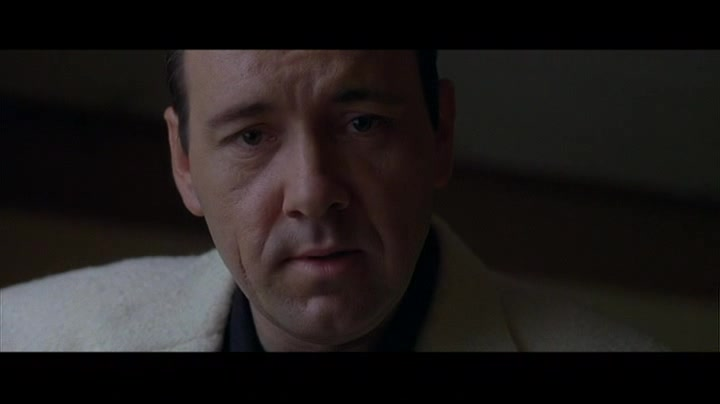
\includegraphics[width=0.98\linewidth]
    {fig/slightLeft.jpg}
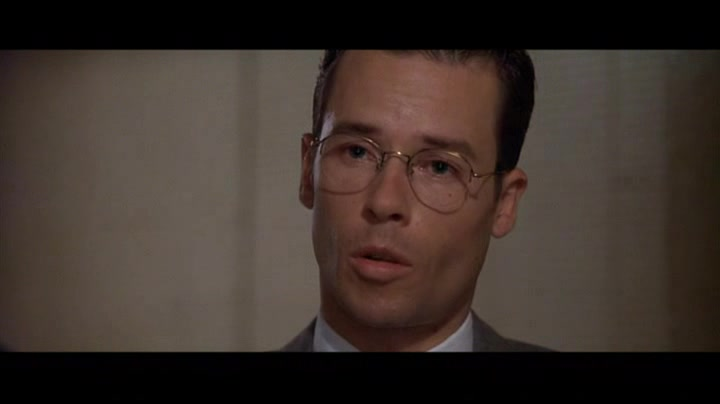
\includegraphics[width=0.98\linewidth]
    {fig/slightRight.jpg}
\end{center}
\caption{These faces might both be classified as centered; however, a human viewer can see the relative left \& right positioning of the faces. These subtleties are better captured using a dynamic grid.}
\label{fig:leftRight}
\end{figure}


\begin{figure}
\begin{center}
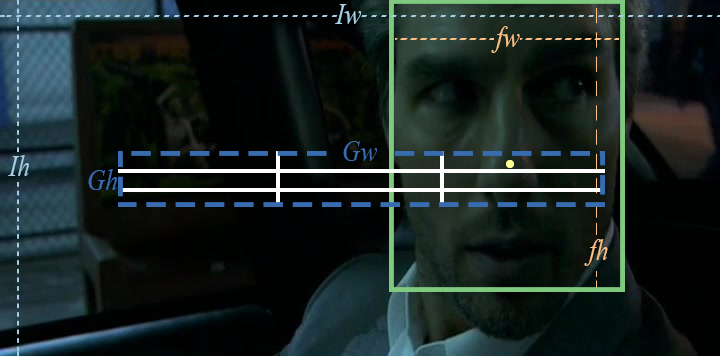
\includegraphics[width=0.98\linewidth]
    {fig/dyGrid.jpg}
\end{center}
\caption{The size of the dynamic grid is based on the size of the face relative to the size of the frame.}
\label{fig:dyGrid}
\end{figure}

\paragraph{The Dynamic Grid}

We use a dynamic grid that  reduces the size of the middle and center sections such that their dimensions are equal to 1/3 of the space in which the facial centroid could occur, see Figure \ref{fig:dyGrid}. The size of the dynamic grid is computed as follows: 

\begin{eqnarray}
  G_{w} &= I_{w} - f_{w} \\
  G_{h} &= I_{h} - f_{h}
\end{eqnarray}

Where $h$ and $w$ represent height and width, respectively, and $G$, $I$, \& $f$ represent Grid, Image, and face. This avoids middle-center convergence, a phenomena where the centroid of large faces converge to the middle-center grid-cell. The dynamic grid  maintains the visual salience of slight position variations (Figure \ref{fig:leftRight}) by preventing middle-center convergence in a principled manner. 
%--------------------------------------------------------------------------------
\begin{figure*}
\begin{center}
\begin{tabular}{c c c c}
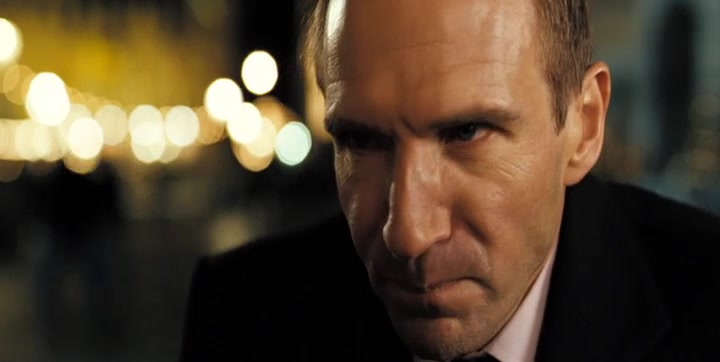
\includegraphics[width=0.22\linewidth]
  {fig/r1.jpg}
& 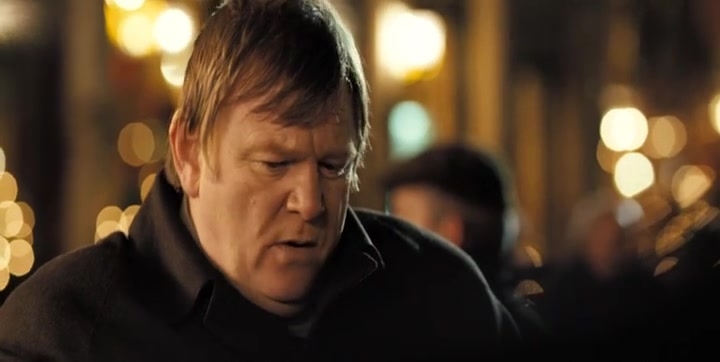
\includegraphics[width=0.22\linewidth]
  {fig/l1.jpg}
& 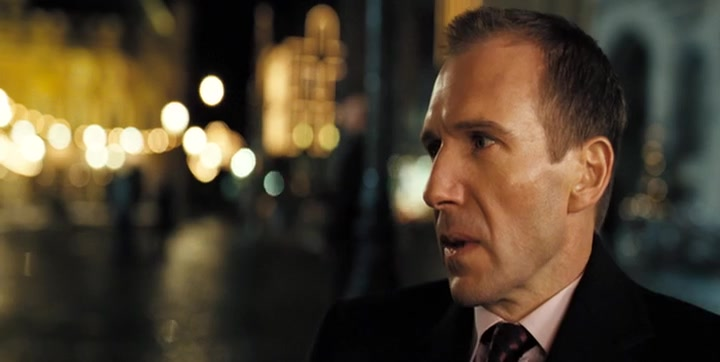
\includegraphics[width=0.22\linewidth]
  {fig/r2.jpg}
& 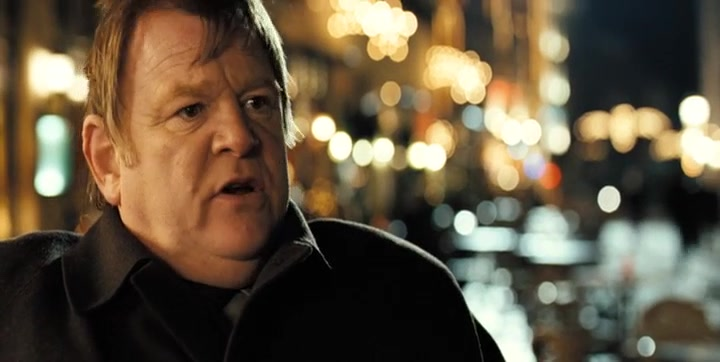
\includegraphics[width=0.22\linewidth]
  {fig/l2.jpg}
\\
\large{1-CU-MR} & \large{1-MCU-ML} & \large{1-CU-MR} & \large{1-MCU-ML} \\
\end{tabular}
\end{center}
   \caption{A proper 2-talk sequence maintains the relative left \& right positioning of the actors from shot to shot. Here we have converted the frame sequence into a string: \textit{1-CU-MR, 1-MCU-ML, 1-CU-MR, 1-MCU-ML.}}
\label{fig:2talk}
\end{figure*}


\subsection{The Sequence}
We define a sequence as a series of frames of arbitrary length. Scenes are then a subset of sequences that fit within the single idea constraint. Defining a sequence as a series of frames with or without scene continuity allows us to search for patterns of frames that are frequently used to construct sequences. One example of this kind of pattern is that used in a 2-actor dialogue. One common construction of a scene in which two actors converse is to place one actor in the right side of the frame and the other actor in the left side of the frame. The frames alternate from showing one actors face to the other, but the relative positioning remains the same, as in Figure \ref{fig:2talk}. \cite{arijon_grammar_1991} defines many possible shot sequences. We use our frame level classifications to convert the problem of sequence pattern discovery and location into an N-Gram analysis problem.


\begin{figure}
\begin{center}
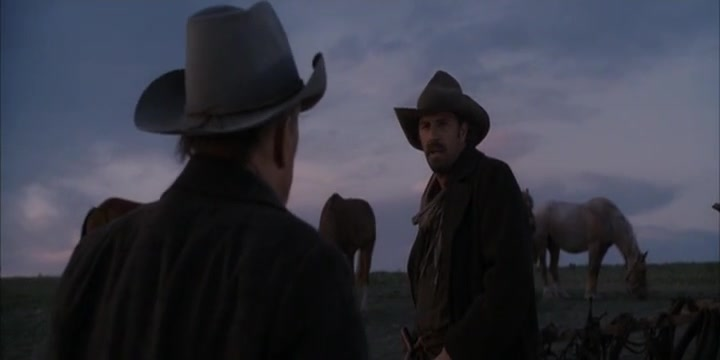
\includegraphics[width=0.98\linewidth]
    {fig/classes/1-MLS-MC.jpg}

\large{1-MLS-MC}
\caption{Frame converted to string: \textit{1 Face - Medium Long Shot - Middle Center}}
\end{center}
\label{fig:tagExample1}
\end{figure}

\begin{figure}
\begin{center}
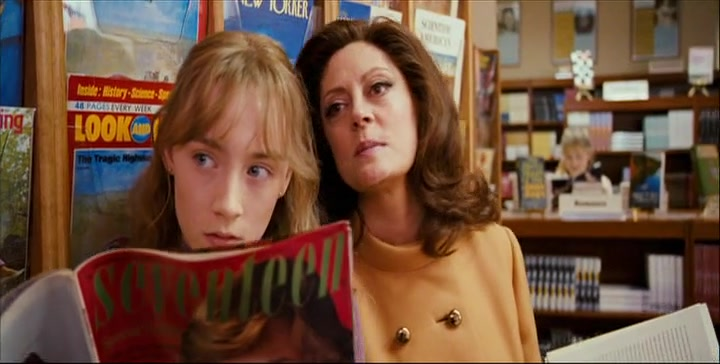
\includegraphics[width=0.98\linewidth]
    {fig/classes/2-MCU-TC.jpg}

\large{2-MCU-TC}
\caption{Frame converted to string: \textit{2 Faces - Medium Close-Up - Top Center}. The bounding box for the face in the back of this image is larger than the one for the face in the front. This results in position being classified by her location.}
\end{center}
\label{fig:tagExample2}
\end{figure}


%--------------------------------------------------------------------------------
\subsection{Identifying \& Locating Patterns}
Understanding the visual impact of these sequence structures is best illustrated by the idea of the two person dialogue or '2-talk'. When filming these kinds of sequences, the cinematographer defines the line of interest as the line between the eyes of the two actors, see Figure \ref{fig:lineOfInterest}. The cinematographer places all of the cameras to one side of this line of interest. This significantly reduces the possibility that cameras will appear in each other's image planes. More relevant to our work, it maintains position consistency of the two actors from frame to frame, see Figure \ref{fig:2talk}. 

The 2-talk and other scene and sequence patterns are a key element in cinematographic style. The patterns defined in \cite{arijon_grammar_1991} and other cinematographic textbooks are often what differentiates a professionally filmed motion-picture from what one might see on YouTube. In the frame classification step, we tagged each frame based on its population, zoom, and position. With these tags, we convert a frame into a string as shown in Figure \ref{fig:2talk}. We then define a motion-picture as a string with many such frames. This reduces the problem of visual pattern finding to one of N-Gram analysis.


\begin{figure}
\begin{center}
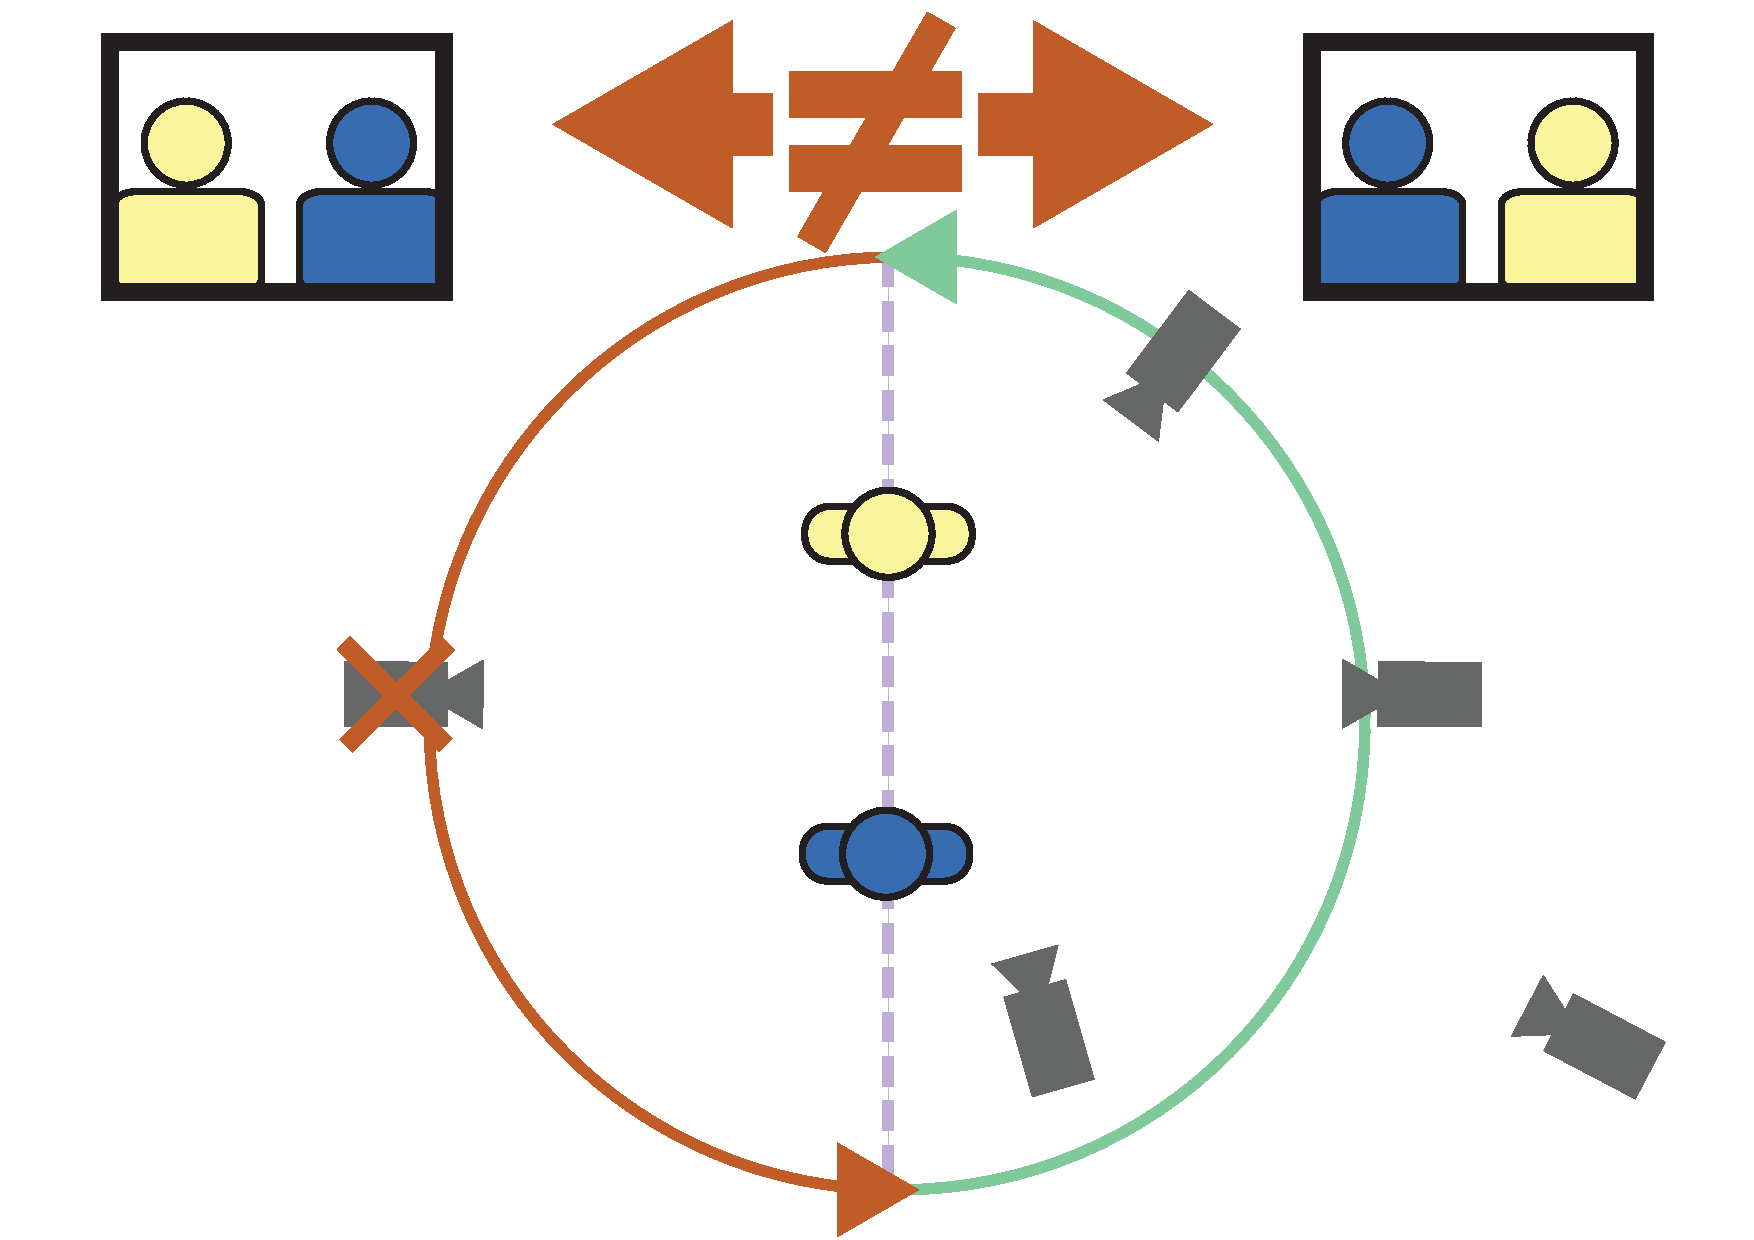
\includegraphics[width=0.98\linewidth]
    {fig/lineOfAction.pdf}
\end{center}
\caption{By placing all cameras on one side of the invisible 'line of interest' for an entire scene, the relative positioning of actors will remain consistent from shot to shot.}
\label{fig:lineOfInterest}
\end{figure}

%--------------------------------------------------------------------------------
\subsubsection{N-Gram Analysis}
We reduce our visual pattern finding problem into one of text analysis and use simple N-Gram algorithms to find visual patterns. The primary algorithm we use is most frequent substring. Having defined each movie in a dataset as a string of frame-tags, we pass the set of strings into the algorithm. We also define a minimum length, a maximum length, and a minumum or maximum number of repetitions. The system outputs a list of all patterns that meet our length and repetition critera and their frequency within the dataset. If we have a known pattern, whether selected from a cinematography text or found through our pattern discovery tool, we use simple text-search tools to find which movies contain that pattern and where the pattern occurs. Figures \ref{fig:pat1} shows still-frame examples of a single pattern found in multiple movies.

Without an effective shot detector, our framework relies on frame by frame sequence analysis. Because the likelihood of any two shots having exactly the same length is very small, we allow for duration invariance in our sequence analysis. To support this, we compress the movie strings such that each element in the string is different than those adjacent to it. With the addition of an effective shot detector and a larger database of movies, it will be informative to compare movies both with and without this duration invariance.
%--------------------------------------------------------------------------------



\section{Results}

\begin{figure}
\begin{center}
\begin{tabular}{cccc}
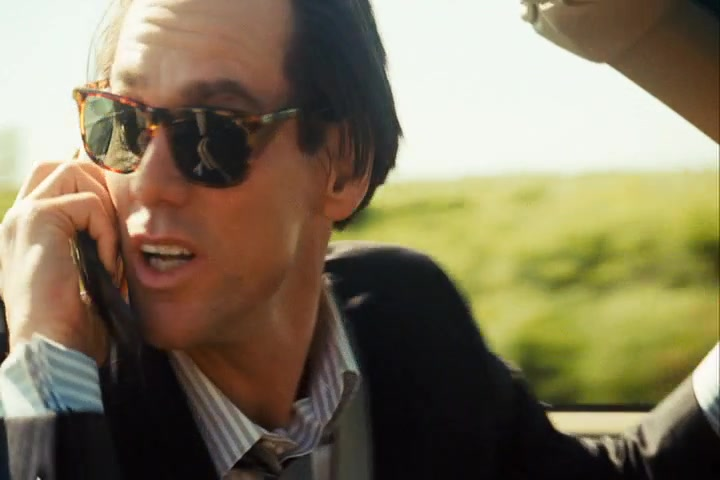
\includegraphics[width=0.2\linewidth]
  {fig/close-ups/01.jpg} 
& 
\includegraphics[width=0.2\linewidth]
  {fig/close-ups/02.jpg}  
& 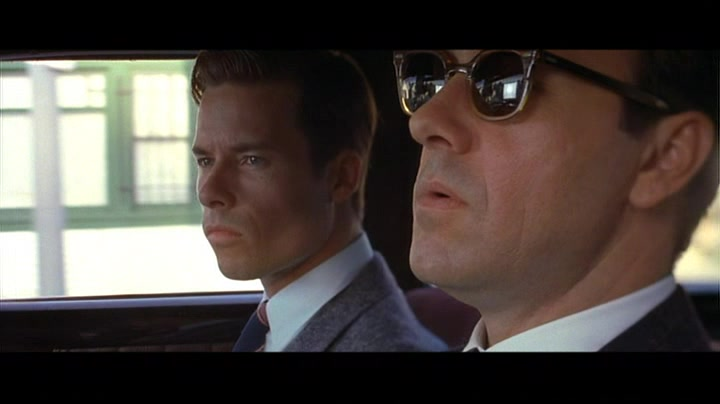
\includegraphics[width=0.2\linewidth]
  {fig/close-ups/10.jpg}   
& 
\includegraphics[width=0.2\linewidth]
  {fig/close-ups/15.jpg}
\\
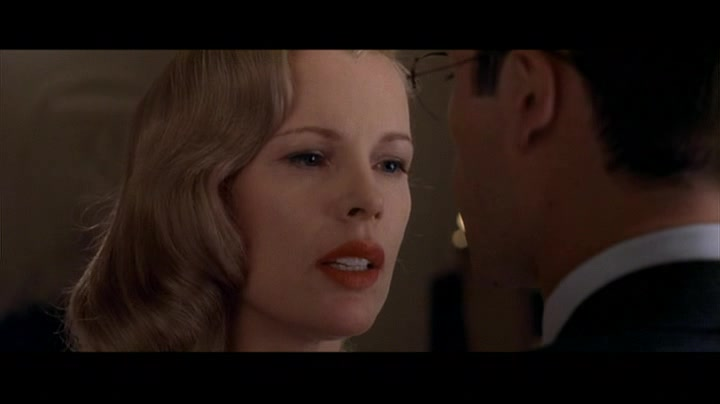
\includegraphics[width=0.2\linewidth]
  {fig/close-ups/05.jpg} 
& 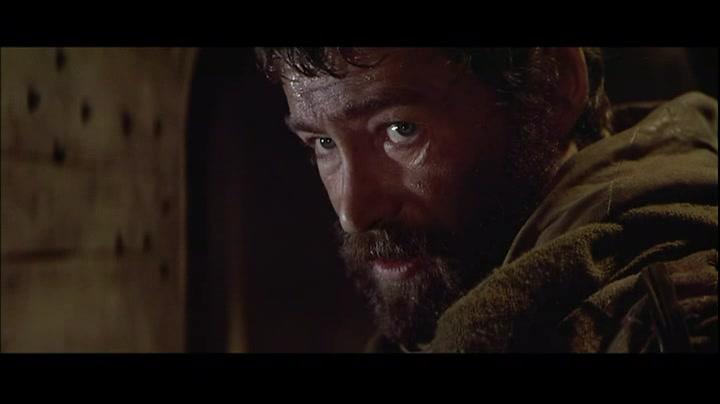
\includegraphics[width=0.2\linewidth]
  {fig/close-ups/06.jpg}  
& 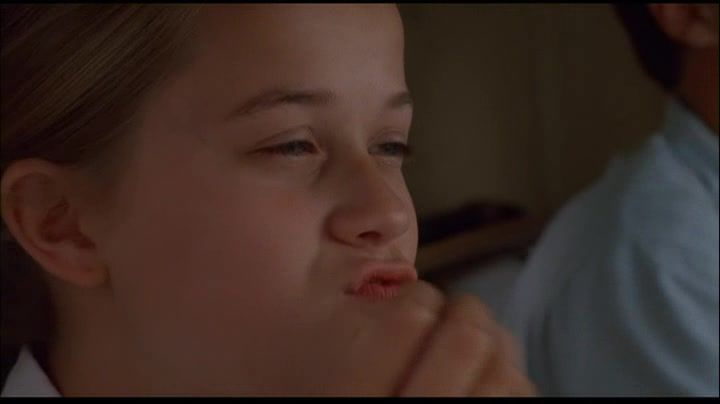
\includegraphics[width=0.2\linewidth]
  {fig/close-ups/07.jpg}   
& 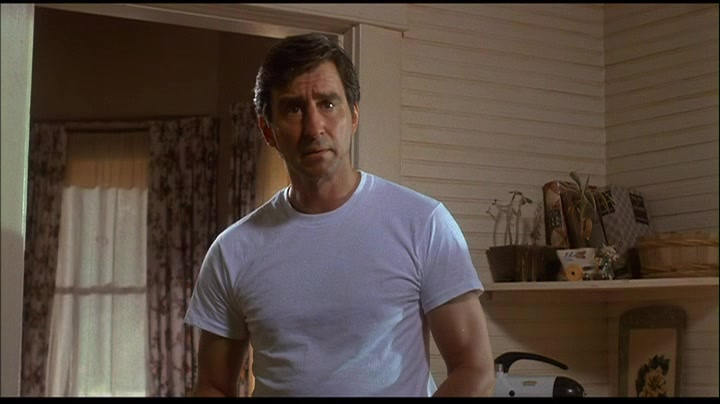
\includegraphics[width=0.2\linewidth]
  {fig/close-ups/08.jpg}
\\

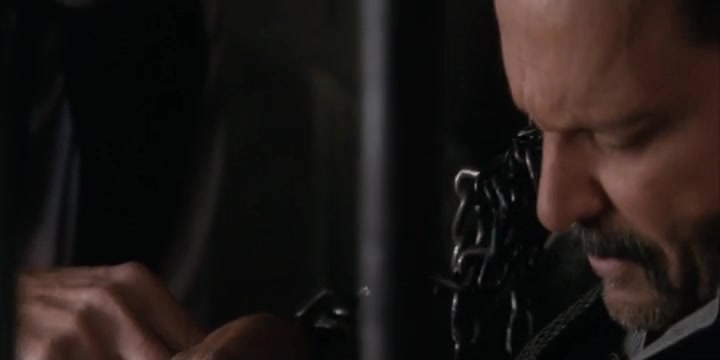
\includegraphics[width=0.2\linewidth]
  {fig/close-ups/09.jpg} 
& 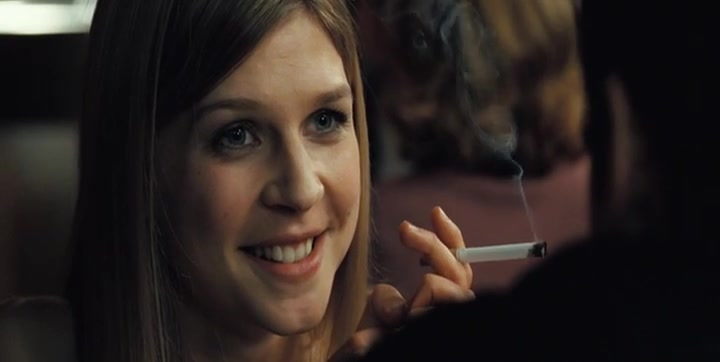
\includegraphics[width=0.2\linewidth]
  {fig/close-ups/04.jpg}  
& 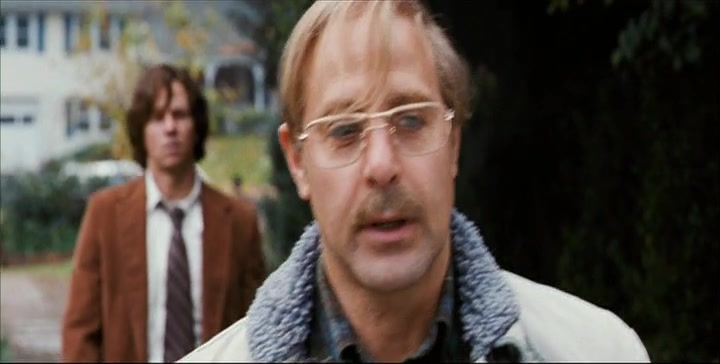
\includegraphics[width=0.2\linewidth]
  {fig/close-ups/11.jpg}   
& 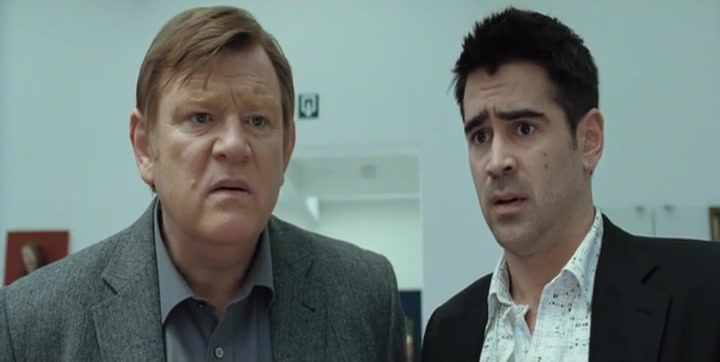
\includegraphics[width=0.2\linewidth]
  {fig/close-ups/12.jpg}
\\
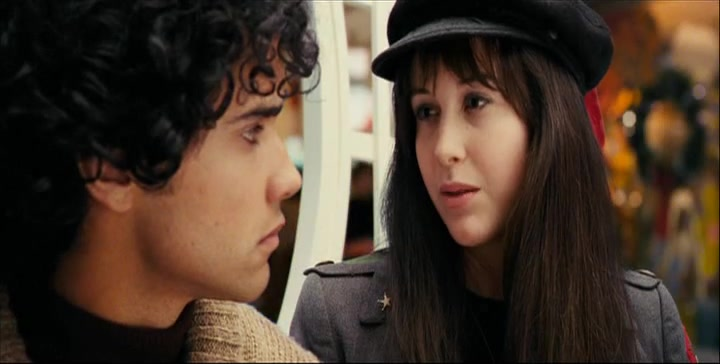
\includegraphics[width=0.2\linewidth]
  {fig/close-ups/13.jpg} 
& 
\includegraphics[width=0.2\linewidth]
  {fig/close-ups/14.jpg}  
& 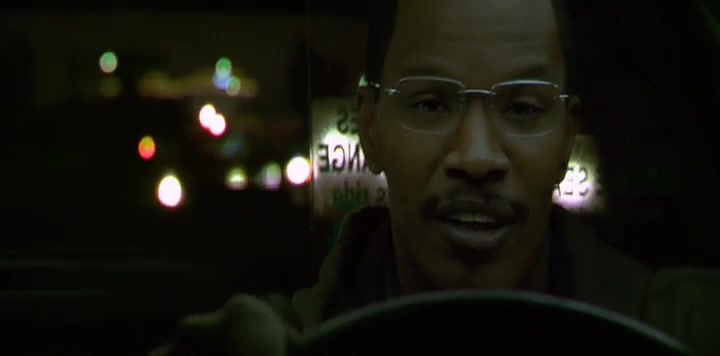
\includegraphics[width=0.2\linewidth]
  {fig/close-ups/03.jpg}   
& 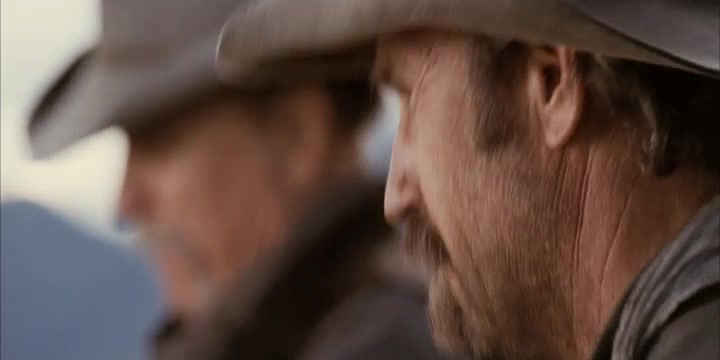
\includegraphics[width=0.2\linewidth]
  {fig/close-ups/16.jpg}
\\
\end{tabular}
\end{center}
   \caption{Example Close-Ups found in our dataset.}
\label{fig:closeUps}
\end{figure}



\begin{figure}
\begin{center}
\begin{tabular}{cccc}
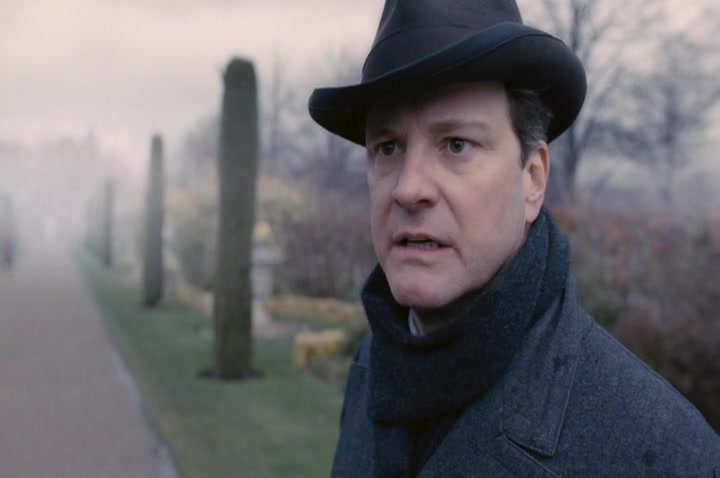
\includegraphics[width=0.2\linewidth]
  {fig/pos/08.jpg} 
& 
\includegraphics[width=0.2\linewidth]
  {fig/pos/02.jpg}  
& 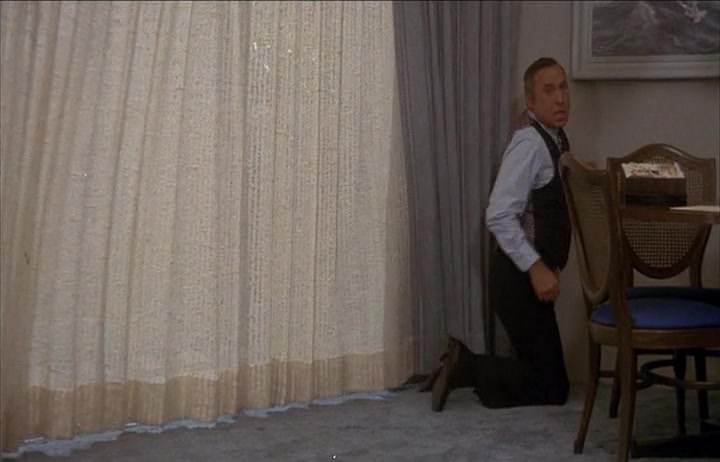
\includegraphics[width=0.2\linewidth]
  {fig/pos/12.jpg}   
& 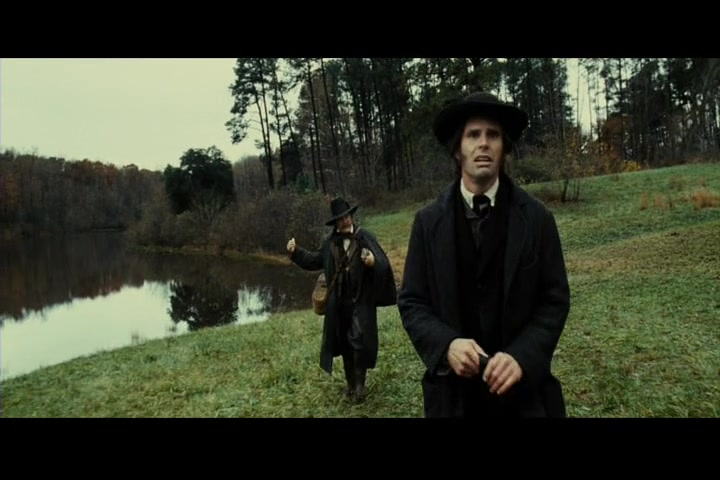
\includegraphics[width=0.2\linewidth]
  {fig/pos/11.jpg}
\\
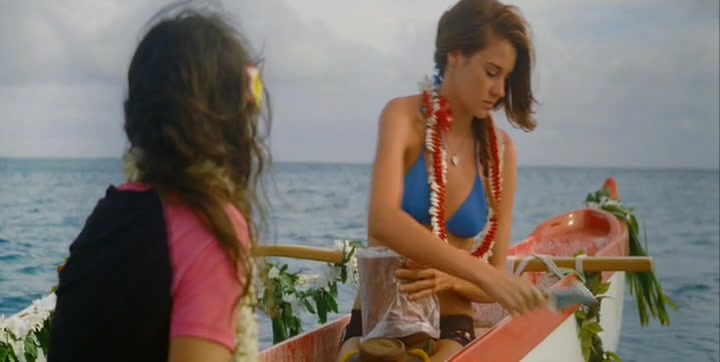
\includegraphics[width=0.2\linewidth]
  {fig/pos/05.jpg} 
& 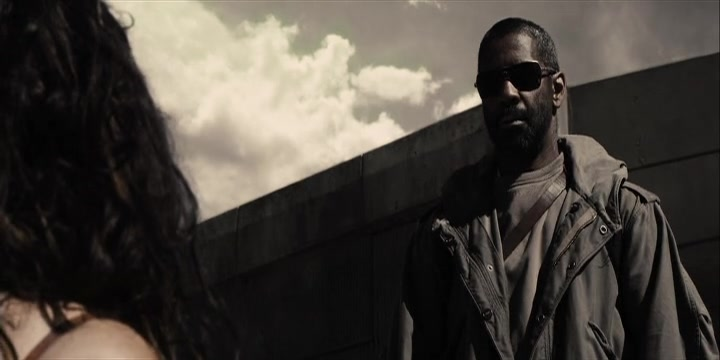
\includegraphics[width=0.2\linewidth]
  {fig/pos/06.jpg}  
& 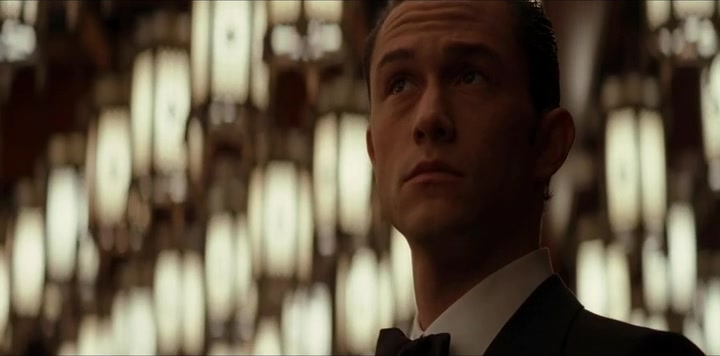
\includegraphics[width=0.2\linewidth]
  {fig/pos/07.jpg}   
& 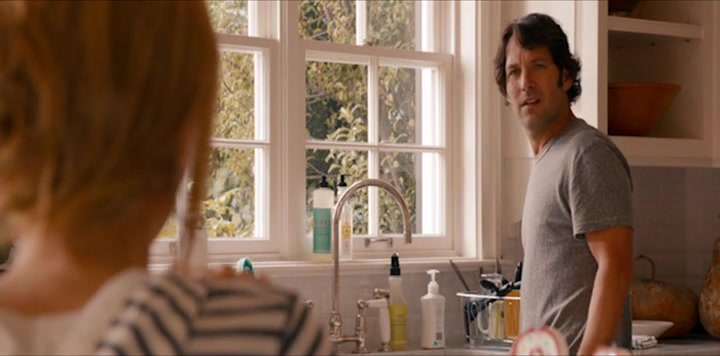
\includegraphics[width=0.2\linewidth]
  {fig/pos/01.jpg}
\\

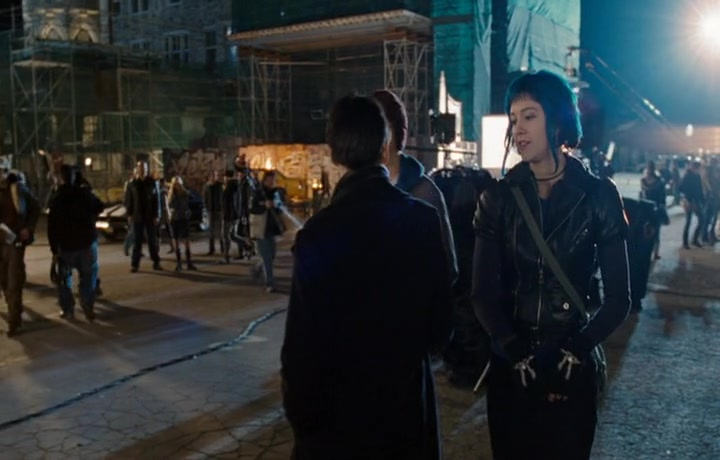
\includegraphics[width=0.2\linewidth]
  {fig/pos/09.jpg} 
& 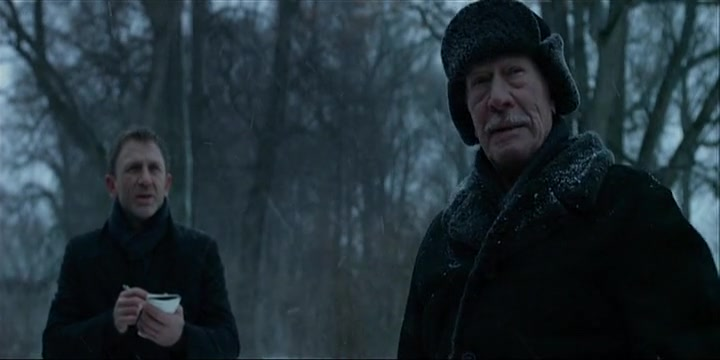
\includegraphics[width=0.2\linewidth]
  {fig/pos/04.jpg}  
& 
\includegraphics[width=0.2\linewidth]
  {fig/pos/15.jpg}   
& 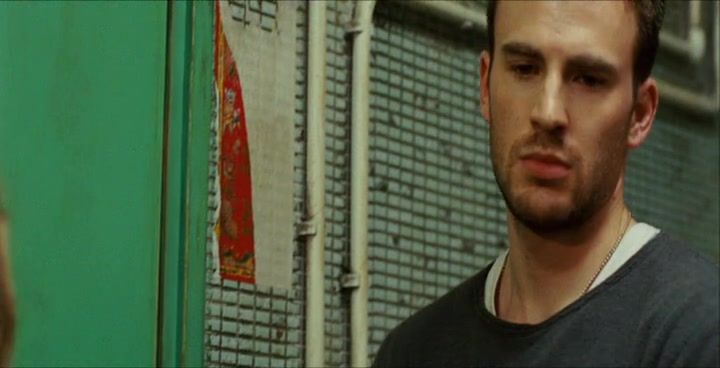
\includegraphics[width=0.2\linewidth]
  {fig/pos/10.jpg}
\\
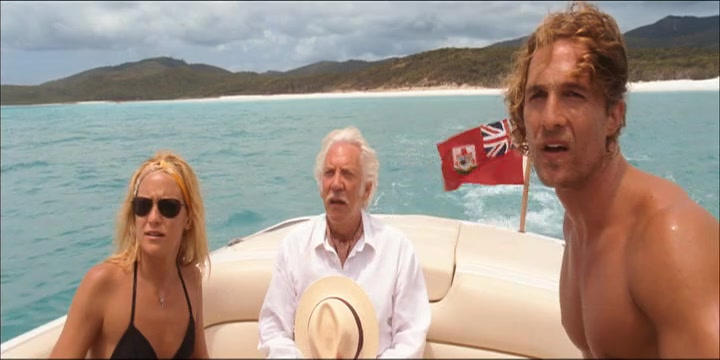
\includegraphics[width=0.2\linewidth]
  {fig/pos/13.jpg} 
& 
\includegraphics[width=0.2\linewidth]
  {fig/pos/14.jpg}  
& 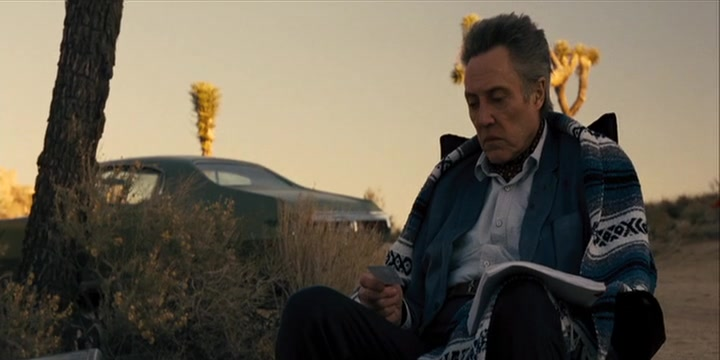
\includegraphics[width=0.2\linewidth]
  {fig/pos/03.jpg}   
& 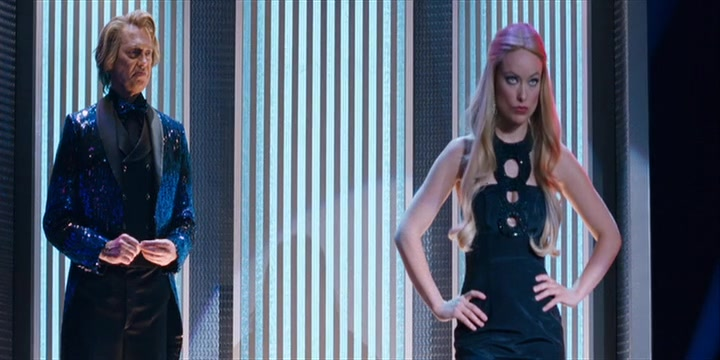
\includegraphics[width=0.2\linewidth]
  {fig/pos/16.jpg}
\\
\end{tabular}
\end{center}
   \caption{Example frames with faces in the Top Right.}
\label{fig:topRight}
\end{figure}


\begin{figure}
\begin{center}
\begin{tabular}{cccc}
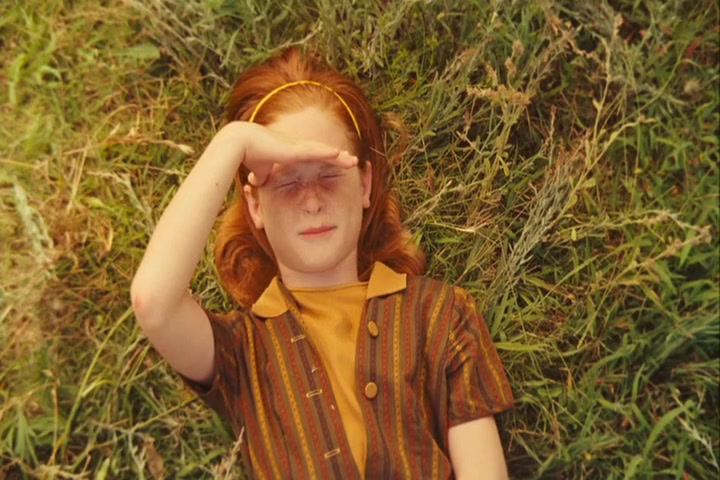
\includegraphics[width=0.2\linewidth]
  {fig/clust/05.jpg} 
& 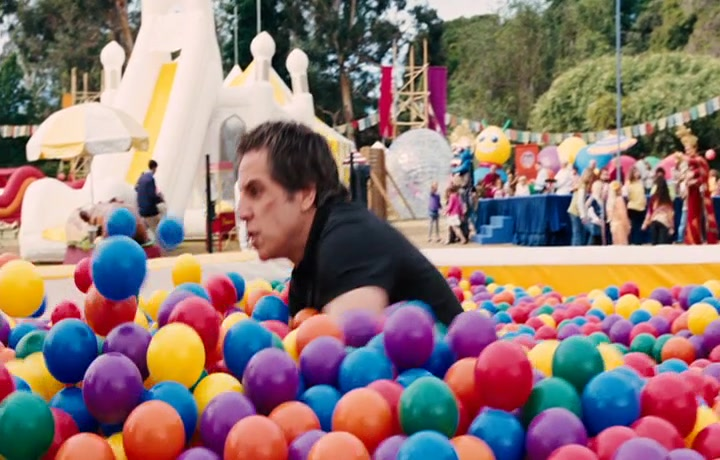
\includegraphics[width=0.2\linewidth]
  {fig/clust/07.jpg}  
& 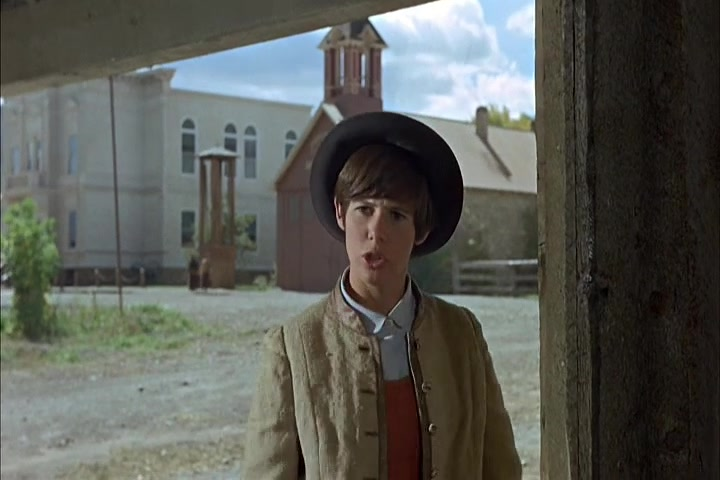
\includegraphics[width=0.2\linewidth]
  {fig/clust/13.jpg}   
& 
\includegraphics[width=0.2\linewidth]
  {fig/clust/14.jpg}
\\
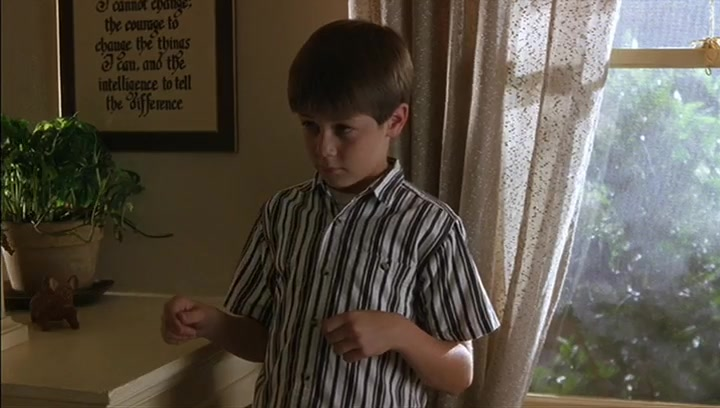
\includegraphics[width=0.2\linewidth]
  {fig/clust/01.jpg} 
& 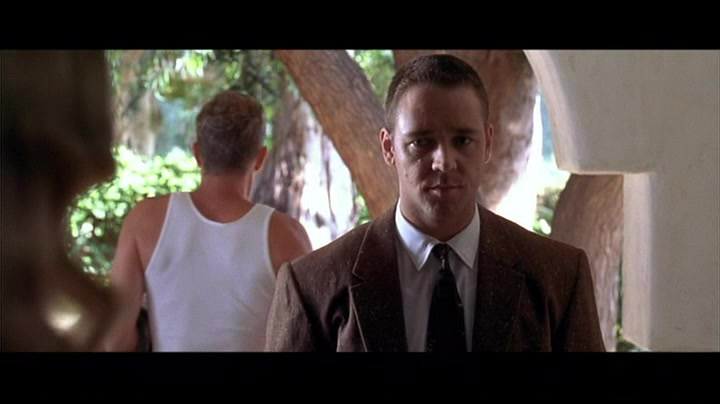
\includegraphics[width=0.2\linewidth]
  {fig/clust/06.jpg}  
& 
\includegraphics[width=0.2\linewidth]
  {fig/clust/02.jpg}   
& 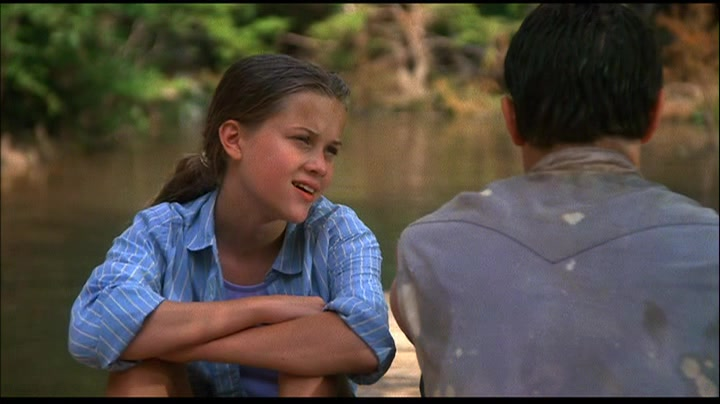
\includegraphics[width=0.2\linewidth]
  {fig/clust/08.jpg}
\\

\includegraphics[width=0.2\linewidth]
  {fig/clust/09.jpg} 
& \includegraphics[width=0.2\linewidth]
  {fig/clust/10.jpg}  
& \includegraphics[width=0.2\linewidth]
  {fig/clust/11.jpg}   
& \includegraphics[width=0.2\linewidth]
  {fig/clust/12.jpg}
\\
\includegraphics[width=0.2\linewidth]
  {fig/clust/03.jpg} 
& \includegraphics[width=0.2\linewidth]
  {fig/clust/04.jpg}  
& \includegraphics[width=0.2\linewidth]
  {fig/clust/15.jpg}   
& \includegraphics[width=0.2\linewidth]
  {fig/clust/16.jpg}
\\
\end{tabular}
\end{center}
   \caption{Example Frames classified as 1-MS-MC}
\label{fig:cluster}
\end{figure}

Figure \ref{fig:closeUps} shows examples of close-ups found in our dataset.
Figure \ref{fig:topRight} shows examples of frames classified as 'Top Right'. Each frame has a face in the upper right region.
Figure \ref{fig:cluster} shows multiple frames that share the same population, zoom, \& position.
%--------------------------------------------------------------------------------

\begin{figure*}
\begin{center}
\begin{tabular}{c c c c c c c}
\includegraphics[width=0.11\linewidth]
  {fig/pat1/breach/01.jpg}
& \includegraphics[width=0.11\linewidth]
  {fig/pat1/breach/02.jpg}
& \includegraphics[width=0.11\linewidth]
  {fig/pat1/breach/03.jpg}
& \includegraphics[width=0.11\linewidth]
  {fig/pat1/breach/04.jpg}
& \includegraphics[width=0.11\linewidth]
  {fig/pat1/breach/05.jpg}
& \includegraphics[width=0.11\linewidth]
  {fig/pat1/breach/06.jpg}
& \includegraphics[width=0.11\linewidth]
  {fig/pat1/breach/07.jpg}
\\

\includegraphics[width=0.11\linewidth]
  {fig/pat1/dinnerForSchmucks/01.jpg}
& \includegraphics[width=0.11\linewidth]
  {fig/pat1/dinnerForSchmucks/02.jpg}
& \includegraphics[width=0.11\linewidth]
  {fig/pat1/dinnerForSchmucks/03.jpg}
& \includegraphics[width=0.11\linewidth]
  {fig/pat1/dinnerForSchmucks/04.jpg}
& \includegraphics[width=0.11\linewidth]
  {fig/pat1/dinnerForSchmucks/05.jpg}
& \includegraphics[width=0.11\linewidth]
  {fig/pat1/dinnerForSchmucks/06.jpg}
& \includegraphics[width=0.11\linewidth]
  {fig/pat1/dinnerForSchmucks/07.jpg}
\\

\includegraphics[width=0.11\linewidth]
  {fig/pat1/gangsterSquad/01.jpg}
& \includegraphics[width=0.11\linewidth]
  {fig/pat1/gangsterSquad/02.jpg}
& \includegraphics[width=0.11\linewidth]
  {fig/pat1/gangsterSquad/03.jpg}
& \includegraphics[width=0.11\linewidth]
  {fig/pat1/gangsterSquad/04.jpg}
& \includegraphics[width=0.11\linewidth]
  {fig/pat1/gangsterSquad/05.jpg}
& \includegraphics[width=0.11\linewidth]
  {fig/pat1/gangsterSquad/06.jpg}
& \includegraphics[width=0.11\linewidth]
  {fig/pat1/gangsterSquad/07.jpg}
\\

\includegraphics[width=0.11\linewidth]
  {fig/pat1/inBruges/01.jpg}
& \includegraphics[width=0.11\linewidth]
  {fig/pat1/inBruges/02.jpg}
& \includegraphics[width=0.11\linewidth]
  {fig/pat1/inBruges/03.jpg}
& \includegraphics[width=0.11\linewidth]
  {fig/pat1/inBruges/04.jpg}
& \includegraphics[width=0.11\linewidth]
  {fig/pat1/inBruges/05.jpg}
& \includegraphics[width=0.11\linewidth]
  {fig/pat1/inBruges/06.jpg}
& \includegraphics[width=0.11\linewidth]
  {fig/pat1/inBruges/07.jpg}
\\

\includegraphics[width=0.11\linewidth]
  {fig/pat1/theBookOfEli/01.jpg}
& \includegraphics[width=0.11\linewidth]
  {fig/pat1/theBookOfEli/02.jpg}
& \includegraphics[width=0.11\linewidth]
  {fig/pat1/theBookOfEli/03.jpg}
& \includegraphics[width=0.11\linewidth]
  {fig/pat1/theBookOfEli/04.jpg}
& \includegraphics[width=0.11\linewidth]
  {fig/pat1/theBookOfEli/05.jpg}
& \includegraphics[width=0.11\linewidth]
  {fig/pat1/theBookOfEli/06.jpg}
& \includegraphics[width=0.11\linewidth]
  {fig/pat1/theBookOfEli/07.jpg}
\\

\includegraphics[width=0.11\linewidth]
  {fig/pat1/theGirlWithTheDragonTatoo/01.jpg}
& \includegraphics[width=0.11\linewidth]
  {fig/pat1/theGirlWithTheDragonTatoo/02.jpg}
& \includegraphics[width=0.11\linewidth]
  {fig/pat1/theGirlWithTheDragonTatoo/03.jpg}
& \includegraphics[width=0.11\linewidth]
  {fig/pat1/theGirlWithTheDragonTatoo/04.jpg}
& \includegraphics[width=0.11\linewidth]
  {fig/pat1/theGirlWithTheDragonTatoo/05.jpg}
& \includegraphics[width=0.11\linewidth]
  {fig/pat1/theGirlWithTheDragonTatoo/06.jpg}
& \includegraphics[width=0.11\linewidth]
  {fig/pat1/theGirlWithTheDragonTatoo/07.jpg}
\\

\includegraphics[width=0.11\linewidth]
  {fig/pat1/thisIs40/01.jpg}
& \includegraphics[width=0.11\linewidth]
  {fig/pat1/thisIs40/02.jpg}
& \includegraphics[width=0.11\linewidth]
  {fig/pat1/thisIs40/03.jpg}
& \includegraphics[width=0.11\linewidth]
  {fig/pat1/thisIs40/04.jpg}
& \includegraphics[width=0.11\linewidth]
  {fig/pat1/thisIs40/05.jpg}
& \includegraphics[width=0.11\linewidth]
  {fig/pat1/thisIs40/06.jpg}
& \includegraphics[width=0.11\linewidth]
  {fig/pat1/thisIs40/07.jpg}
\\
\large{1-MCU-L} & \large{1-MCU-R} 
& \large{1-MCU-L} & \large{1-MCU-R} 
& \large{1-MCU-L} & \large{1-MCU-R} 
& \large{1-MCU-L} \\

\end{tabular}
\end{center}
\label{fig:pat1}
\end{figure*}

Figures \ref{fig:pat1} \& \ref{fig:pat2} show still-frame examples of a pattern occurring in several different movies from our dataset. 


\begin{center}
  \begin{tabular}{ l | r r }
    Movie Clip & Precision \% & Recall \% \\
    \hline
    \textit{ Back To The Future III } &  83.19 &  55.52\\
    \textit{ Breach } &  92.78 &  51.37\\
    \textit{ Broken Flowers } &  92.03 &  4.41\\
    \textit{ Contagion } &  95.98 &  69.09\\
    \textit{ Dazed And Confused } &  80.48 &  11.96\\
    \textit{ Death Proof } &  93.13 &  49.76\\
    \textit{ Dinner For Schmucks } &  73.45 &  23.30\\
    \textit{ Escape From Alcatraz } &  95.16 &  47.91\\
    \textit{ Gosford Park } &  95.27 &  1.94\\
    \textit{ Salt } &  85.42 &  57.66\\
    \textit{ Super 8 } &  84.35 &  49.74\\
    \textbf{ Average } &  \textbf{89.39} &  \textbf{38.63}\\
    \label{tab:shotdetResults}
  \end{tabular}
\end{center}
    
%%%%%%%%%%%%%%%%%%%%%%%%%%%%%%

%--------------------------------------------------------------------------------
\subsection{Detectors}
%--------------------------------------------------------------------------------
\subsubsection{Face Detection}
Our current system uses the HeadHunter \cite{mathias_face_2014} detection model as formulated for the Deformable Parts Model \cite{lsvm-pami}. While not quite reaching the performance of the current state-of-the-art, this detector is available off the shelf and can be run on remote clusters with little setup cost. As better face detectors become available, we will incorporate them into our framework.

%--------------------------------------------------------------------------------
\subsubsection{Shot Detection}
Shot boundary detection looks to computationally identify the moments when one shot transitions to another. This is a very well studied problem \cite{boreczky1996comparison} \cite{lienhart1998comparison} \cite{lu2013fast} \cite{chavan2014review} and was a primary task in TrecVid's yearly competition \cite{smeaton_video_2010} through 2006. Table \ref{tab:shotdetResults} compares the performance of the best off-the-shelf shot boundary detector, Shotdetect \cite{mathe_shotdetect_2015}, with a ground-truth dataset created manually for several of the movies on our dataset, allowing for variance of up to 0.4 seconds. Based on these results, we elected to save shot based analyses to future work when we either get a better off-the-shelf shot detector or implement the state-of-the-art. An ideal shot detector has (1) High precision/Recall for both hard and gradual cuts, (2) Robustness to large changes in scene, (3) Robustness to camera motion, \& (4) Consistent location for gradual cuts (e.g. always at the halfway point between to shots).
